\chapter{Literature Review}% Main chapter title
\thispagestyle{nohead}
\label{LitReview} % For referencing the chapter elsewhere, use \ref{LitReview} 

%----------------------------------------------------------------------------------------

\where incorporates ideas from at least three separate disciplines: software verification, machine learning, and software measurement and metrics. Each of these disciplines has a considerable body of research associated with it.
A Venn diagram illustrating how the literature was classified is given in Figure \ref{fig:litreview}. 
%It can be seen that the intersection of \textit{software verification} and \textit{measurement/metrics} itself contains two separate categories of interest: benchmarks and competitions in formal methods, and the relatively young field of \textit{proof engineering}.
We shall concentrate this review on Software Verification and its intersections with other domains relevant to this project; i.e. Sections \ref{sec:lrsv}, \ref{sub:lrsvmm}, \ref{sub:lrsvml}, and \ref{sub:lrsvmmml}. 
The rest of this chapter will review the literature associated with each segment of Figure \ref{fig:litreview} - moving clockwise from the top.


\begin{figure}

\centering
\def\firstcircle{(3cm,0cm) circle (2.5cm)}
\def\secondcircle{(0cm,0cm) circle (2.5cm)}
\def\thirdcircle{(1.5cm,3cm) circle (2.5cm)}
% Suppose we have three circles or ellipses or whatever. Let us define
% commands for their paths since we will need them repeatedly in the
% following:
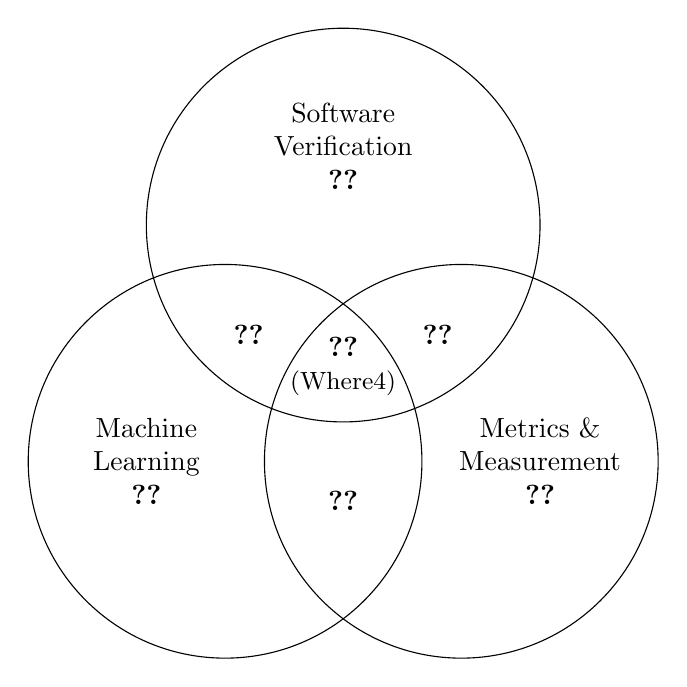
\begin{tikzpicture}
	
	\draw \firstcircle node [below] {};
	\draw \secondcircle node [above] {};
	\draw \thirdcircle node [below] {};
	\node[align=center] at (-1cm, 0cm) {Machine\\Learning\\ \ref{sec:lrml} };
	\node[align=center] at (1.5cm, 4cm) {Software\\Verification\\ \ref{sec:lrsv}};
	\node[align=center] at (4cm, 0cm) {Metrics \&\\ Measurement\\ \ref{sec:lrmm}};
	\node[align=center] at (1.5cm, 1.2cm) {\ref{sub:lrsvmmml}\\\small{(Where4)} };
	\node[align=center] at (0.3cm, 1.6cm) {\ref{sub:lrsvml}};
	\node[align=center] at (2.7cm, 1.6cm) {\ref{sub:lrsvmm}};
	\node[align=center] at (1.5cm, -0.5cm) {\ref{sub:lrmmml}};
	
\end{tikzpicture}

\caption{\where as placed at the intersection of three disciplines}
\label{fig:litreview}

\end{figure}


\section{\why and Software Verification Systems}
\label{sec:lrsv}

An overview of the \why verification system \cite{why:shephard,why:whereprovers} has been given in the previous chapter. The WhyML programming language provides a high-level ML\footnote{The ML language - not to be confused with \underline{M}achine \underline{L}earning}-like language for the specification of programs with pre- and post- conditions, recursive definitions and type invariants. An extensive library of verified polymorphic data-types make WhyML a flexible language \cite{verifythis,why:polymorphic}. As we stated in the previous chapter, it is \why's driver-based approach to interfacing with external tools that is of most interest to our project. The \why approach is, in this regard, quite different from the typical SV system of tightly-integrated systems consisting of an IDE/annotation language/front-end DSL, intermediate logic language, and SMT-solving back-end. Examples of systems which follow this latter model are Spec\# \cite{spec} and Dafny \cite{Dafny} which use the Boogie \cite{Boogie} intermediate language and the Z3 \cite{Z3} SMT solver.

The diversity of languages and formalisms has been matched by an increase in software verification \textit{tools} in recent years. Filli{\^a}tre's overview of the deductive verification tool landscape \cite{deductiveSV} counts 65 tools cited or used in the five papers of a special edition of the \textit{Verified Software: Theory, Tools and Experiments} workshop. Recently, there has been an effort to make these tools more interoperable. The two-dozen ATPs, ITPs and SMT solvers targeted by \why make it an attractive choice for translations: recent projects have used \why as a platform for discharging POs translated from Boogie \cite{b2w} and the B system \cite{rodinplugin,atelierB2w}. 

\subsection{Measurement and Metrics in Software Verification}
\label{sub:lrsvmm}

With the diversity of approaches currently in use in the SV domain, experimental software measurement concepts and techniques must be introduced for the rigorous evaluation, comparison, and characterisation of software. These techniques are usually employed in the general software engineering domain and have been adapted for the specific concerns of formal methods. 

The intersection of SV and empirical SE disciplines can be further broken into the three subsections to follow.      

\subsubsection{Software Verification Competitions}
\label{sub:lrsvmmbench}

At present, competitions provide the most prominent means of comparing systems which focus on the verification of object-oriented software. In competitions such as those held at FoVeOOS 2011 \cite{bormer:hal-00789525} and the VerifyThis series \cite{Huisman2015}, teams are given the natural-language specifications and pseudo-code for a small number of typical SV problems. Any system can be used, with tool developers often choosing to compete using their own system. Many of the \why gallery of verified programs originated from software verification competitions \cite{verifythis, tafat:inria-00636083} . 

The competitive environment for automatic program verifiers (which use model-checking techniques to ensure properties such as reachability or termination) is similar: a well-established competition, SV-COMP \cite{SVCOMP}, is held annually. Importantly, a large, publicly-available\footnote{\url{https://github.com/sosy-lab/sv-benchmarks}} benchmark repository consisting of 6661 programs \cite{Beyer2016} has been developed using these competition questions. It is possible to maintain such a repository due to the standard input format of the tools which all accept input in the C language. Other efforts to standardise benchmark repositories for software verification tools are discussed in the next subsection.  

\subsubsection{Benchmark Repositories}

The need for a standard set of benchmarks for the diverse range of verification systems was identified by a number of participants in the week-long seminar at Dagstuhl \cite{Dagstuhl} in 2014. The series of workshops and events brought the model-checking and SV system communities together. Qualitative, repeatable comparative evaluation was agreed as an important goal if deductive software verification is to advance as an engineering discipline. The VACID-0 \cite{Leino10vacid-0:verification} project is an attempt to maintain a repository of standard abstract specifications for deductive software verification tasks similar to those used in the VerifyThis competition.  

The benefits of such a benchmark suite are identified by the SMT-LIB \cite{SMTLIB} project. The performance of SMT solvers has significantly improved in recent years due in part to the standardisation of an input language and the use of standard benchmark programs in competitions \cite{SMTEVAL2013}. \why uses the SMT-LIB language as input format for a number of SMT solvers (including CVC4 \cite{CVC4}, Z3 \cite{Z3}, and veriT \cite{veriT}). 
%Our previous work \cite{Healy:2016} has exploited this feature to characterise verification tasks  compared to other application domains of SMT solvers.

The TPTP (Thousands of Problems for Theorem Provers) project \cite{TPTP} is a benchmark repository with similar aims to SMT-LIB but a wider scope. The problems target theorem provers which specialise in numerical problems as well as general-purpose SAT and SMT solvers. The TPTP library is specifically designed for the rigorous experimental comparison of solvers \cite{Sutcliffe200139}. There has been significant development effort by \why developers to support the TPTP format in \why and to extend the TPTP language with rank-1 polymorphism \cite{why:tptp}. 

\subsubsection{Proof Engineering}
\label{sub:lrsvmmpe}

The scale of formal software engineering projects has grown in recent years. The formal verification of the seL4 microkernel \cite{Klein:2014:CFV} and Thomas Hales' \textit{FlySpeck} proof of the Kepler Conjecture \cite{hales-kepler} are large and complicated engineering projects developed over a number of years. Both projects represent significant engineering efforts - it is estimated that the seL4 verification took 25 person-years of work - and produced a large volume of software artefacts in the form of \textit{proof scripts}. Researchers applying concepts from software engineering to manage and measure such projects call their practice ``proof engineering'' \cite{Klein2014}.

Both object-oriented software and formal proofs make use of ``modules'' to package related classes and lemmas/axioms respectively. Aspinall and Kaliszyk \cite{Aspinall2016} suggest that this common approach to modularity allows the standard Chidamber and Kemerer \cite{CandK} (CK) metrics to be adapted for formal SE projects. The authors use this analogy to model and measure the dependency tree for proof modules and the derivation of the module's coupling and cohesion metrics (CK metrics will be discussed further in Section \ref{sec:lrmm}).

Other approaches measure syntactic features of the specification to derive complexity metrics. The verification of the seL4 microkernel mentioned previously was used as the basis for at least two similar studies. For this large-scale SV project, the property statement \textit{size} was found to be quadratically related to the human effort (and associated cost) of development \cite{CostIndicator}. Staples et al argue that code sizing (i.e estimating the number of lines of executable C code that will need to be written) is more strongly correlated to the size of the formal specification (both abstract and executable) than to a metric based on a notion of ``function points'' \cite{Staples:2013}.
   
The \textit{quality} of specifications for a single project (the Web-Service Definition Language) was observed over a period of time in a study by Bollin \cite{Zspecs}. In this study, the formal specifications, written in the Z language \cite{Zlang}, were measured for their cohesion and coupling. The measurement of specifications is in contrast to the previous examples \cite{Aspinall2016, CostIndicator} which used the proof scripts.
% This approach is close to the method used to measure \why POs used by \where (as described in Sec. \ref{sub:extracting}).

Formal specification is facilitated by the Object Constraint Language (OCL) in Unified Modelling Language models. Two studies propose complexity metrics for OCL expressions. The first \cite{TowardsOCL} uses structural metrics such as the number of operators, quantifiers, etc. A later study \cite{OCLalt}, however, takes the view that dynamically measuring the \textit{number of objects} involved in the expressions evaluation provides a more accurate measure of complexity.

Proof engineering is a particularly active research area and this brief survey is not definitive. It is intended to give a flavour of work most relevant to \where.     
 
       
\section{Software Measurement and Metrics}
\label{sec:lrmm}
%also include the experimental process
%cite the metrics book
The rigorous measurement of software and the definition of metrics to group and comprehend these measurements is a large area of software engineering in itself. A comprehensive overview of the topic is given in Fenton \& Pfleeger's book \cite{FentonPfleeger}. The metrics of most interest to our project are \textit{internal, structural} code-based metrics. Those introduced in Sec. \ref{sub:extracting} are of this type.

One particularly useful metric for measuring code complexity was defined by McCabe in 1976 \cite{McCabe}. The graph-based cyclomatic complexity of a function is a size-independent and intuitive measure of the code's complexity. It has proved useful in unit-testing scenarios \cite{McCabeTesting}. It is also used to estimate \textit{external} metrics such as how long a project is expected to take, or how much it will cost.  McCabe's complexity metric has previously been adapted for use in measuring the complexity of context-free grammars \cite{nuimeprn6458}. We mapped McCabe's use of decision nodes to the number of conditional operators in \why PO formul\ae.

While structural metrics such as McCabe's are statically measured, the statistically-accurate \textit{dynamic} measurement of software is important if the predicted behaviour of a program is to be related to the \textit{actual} observed behaviour. Many of the associated issues are addressed by Lilja \cite{LiljaJ} in his book on the subject. Robust experimental methods for software engineering are the subject of other major studies \cite{AdvancedESE}, including recent work by Kitchenham et al \cite{Kitchenham2016} who propose the use of kernel density plots as a visualisation method to gain a better understanding of data distribution in the SE domain.

\subsection{Measurement and Machine Learning}
\label{sub:lrmmml}
%mention two journals: Empirical Software Enginnering, one that James said

At the intersection of software metrics, measurement, and machine learning, there has been a growing trend of using ML techniques to make predictions about SE metrics. Examples of this trend include the use of text-based clustering to predict defect resolution time \cite{Assar2016}, effort estimation using SVMs \cite{Song:2014:PBR:2639490.2639510} and the use of genetic algorithms for the efficient allocation of cloud-based resources \cite{cloudML}. In a survey on the topic, Gandotra et al. \cite{ClassificationSurvey} cite numerous examples of the use of ML classification algorithms to identify potentially dangerous or intrusive software. Recent issues of the journals \textit{Empirical Software Engineering} contain many more articles combining the use of ML techniques and standard software metrics.  

\section{Machine Learning}
\label{sec:lrml}

A complete survey of literature in the machine learning domain is far beyond the scope of this or any other thesis. Again, we refer the reader to a useful overview \cite{Mitchell} which balances practical implementation issues for a variety of algorithms with a treatment of their theoretical foundations. We focus this section on some of the background literature and considerations associated with the algorithms compared during the development of \where (Sec. \ref{pred:choosing}).

Our learning task is to predict a continuous-valued variable which makes it a \textit{regression} task in ML terms. More specifically, it is a multi-output regression task as there is one output for each SMT solver. Recommendations regarding the use of SVMs (which excel at \textit{binary} classification) for this task are made by Hsu and Lin \cite{MulticlassSVM}. A More general survey of multi-output regression and how various ML algorithms can either be adapted or extended for this use case is provided by Borchani et al. \cite{multisurvey}. \where uses a Random Forest \cite{RandomForests} method for prediction. The Random Forest approach is an ensemble extension of the Decision Tree \cite{DecisionTrees} algorithm. Both algorithms support multi-output problems natively. More details on the suitability of these algorithms to our problem are given later in the thesis (Sec. \ref{sub:multi}). 

%More broadly, we compare \textit{supervised} machine learning algorithms for use in \where. These algorithms rely on the representation of a ``ground truth''. The         


\subsection{Software Verification and Machine Learning}
\label{sub:lrsvml}

As this project deals with training ML algorithms on software artefacts, it relies on representations of these programs. As discussed in Sec. \ref{sec:lrmm}, the measurement of software requires the use of metrics. The intersection of software verification and machine learning, therefore, necessarily involves concepts from the software metrics and measurement domain. This subsection concentrates on research from the field of interactive theorem proving while the next looks at portfolio solvers in more detail.

We have already introduced the Flyspeck \cite{hales-kepler} proof of the Kepler conjecture. The 14185 theorems and millions of lemmas form the basis for a number of projects which aim to take advantage of ATP tools within interactive environments \cite{Flyspec, Kaliszyk2015109}. These projects involve the translation of TPTP formul\ae~  from the higher-order logic of the  interactive prover \textsf{HOL Light} to the input format of a number of ATPs. Kaliszyk and Urban were also involved with extending Sledgehammer \cite{threeyears} tool for Isabelle \cite{Isabelle} with machine learning capabilities. The MaSh \cite{Sledgehammer} engine uses a Naive Bayes algorithm and clustering to select facts based on syntactic similarity.       

The AI4FM\footnote{\url http://www.ai4fm.org} group includes researchers from Edinburgh, Newcastle and Heriot-Watt universities. Much of the group's work \cite{Heras2013, ML4PG, bundy_et_al:DR:2012:3731} aims use ML/AI to automate the interactive theorem proving process by learning patterns from human experts and proof repositories.  
Other work has performed similar pattern recognition for the ACL2 ITP \cite{Heras2013}. ML4PG (Machine Learning for Proof General) \cite{ML4PG} also uses clustering techniques to guide the user for interactive theorem proving.

\subsection{Where4, portfolio-solving, and the intersection of all three disciplines}
\label{sub:lrsvmmml}

Portfolio-solving approaches have been implemented successfully in the SAT domain by SATzilla \cite{Satzilla} and numerous studies \cite{MUX, DPVZ15:CAV} have used the SVCOMP \cite{SVCOMP} benchmark suite of C programs for model checkers. These particular studies have been predicated on the use of Support Vector Machines (SVM) with only a cursory use of linear regression \cite{MUX}. In this respect, our project represents a more wide-ranging treatment of the various prediction models available for portfolio solving.

\section{Conclusion}
